\let\negmedspace\undefined
\let\negthickspace\undefined
\documentclass[journal,12pt,twocolumn]{IEEEtran}
\usepackage{cite}
\usepackage{amsmath,amssymb,amsfonts,amsthm}
\usepackage{algorithmic}
\usepackage{graphicx}
\usepackage{textcomp}
\usepackage{xcolor}
\usepackage{txfonts}
\usepackage{listings}
\usepackage{enumitem}
\usepackage{mathtools}
\usepackage{gensymb}
\usepackage{comment}
\usepackage[breaklinks=true]{hyperref}
\usepackage{tkz-euclide} 
\usepackage{listings}
\usepackage{gvv}                                        
\def\inputGnumericTable{}                                 
\usepackage[latin1]{inputenc}                                
\usepackage{color}                                            
\usepackage{array}                                            
\usepackage{longtable}                                       
\usepackage{calc}                                             
\usepackage{multirow}                                         
\usepackage{hhline}                                           
\usepackage{ifthen}                                           
\usepackage{lscape}

\newtheorem{theorem}{Theorem}[section]
\newtheorem{problem}{Problem}
\newtheorem{proposition}{Proposition}[section]
\newtheorem{lemma}{Lemma}[section]
\newtheorem{corollary}[theorem]{Corollary}
\newtheorem{example}{Example}[section]
\newtheorem{definition}[problem]{Definition}
\newcommand{\BEQA}{\begin{eqnarray}}
\newcommand{\EEQA}{\end{eqnarray}}
\newcommand{\define}{\stackrel{\triangle}{=}}
\theoremstyle{remark}
\newtheorem{rem}{Remark}
\usepackage{circuitikz}
\begin{document}

\bibliographystyle{IEEEtran}
\vspace{3cm}

\title{GATE-2023, EC-35}
\author{EE23BTECH11033- JASWANTH KILLANA}
\maketitle
\newpage
\bigskip

\renewcommand{\thefigure}{\theenumi}
\renewcommand{\thetable}{\theenumi}
\textbf{Question}:\\
In the circuit shown below, switch S was closed for a long time. If the switch is opened at t=0, the maximum magnitude of the voltage $V_R$ in volts is. (round off to nearest integer).\\

\textbf{solution} :
\begin{figure}[th]
\centering
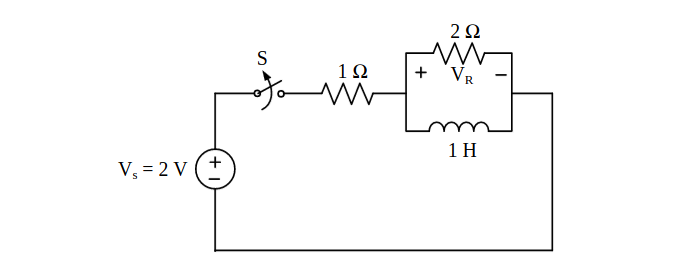
\includegraphics[width=\linewidth]{\root\assign3\figs\gate.png}
\caption{}
\label{}
\end{figure}
\begin{align}
 At, t=0^-
\end{align}
inductor acts as wire\\
apply KVL in big loop
\begin{align}
-2+1i\brak{0^-}&=0\\
i\brak{0^-}&=2A
\end{align}
 \begin{figure}[h!]
   \centering
   \begin{circuitikz}[american]
       \draw (0,3) to [R,a^=$2\ohm$,v=$V_R$](3,3); 
       \draw (0,0) to [short](0,3);
       \draw (3,3) to [short](3,0);
       \draw (0,0) to [L,a^=$1H$,i=$i\brak{t}$] (3,0);
   \end{circuitikz}
   \caption{steady state circuit}
   \end{figure}
here\begin{table}[!ht]
 \centering
  \begin{tabular}{|c|c|c|}
\hline
\textbf{parameter}& \textbf{description}& \textbf{value}
\\\hline
\multirow{3}{1em}\\$l$&length&$50m$
\\\hline
$b$&breadth&$0.25m$
\\\hline
$h$&height&$0.5m$
\\\hline
$y(n)$& sum of volume&$6.25m^3$ 
\\\hline
\end{tabular}


   \caption{input parameters}
   \label{GATE-2023,EC-35}
   \end{table}
   \begin{figure}[h!]
   \centering
   \begin{circuitikz}[american]
       \draw (0,3) to [R,a^=$2\ohm$,v=$V_R$](3,3); 
       \draw (0,0) to [short](0,3);
       \draw (3,3) to [V,a^=$i\brak{0^-}$](3,0);
       \draw (0,0) to [L,a^=$Ls$,i=$I\brak{s}$] (3,0);
   \end{circuitikz}
   \caption{s domain circuit}
   \end{figure}
after t=0,\\
KVL, \begin{align}
2i\brak{t}+L\frac{di}{dt}
\end{align}
apply laplace transform,
\begin{figure}[!ht]
     \centering
     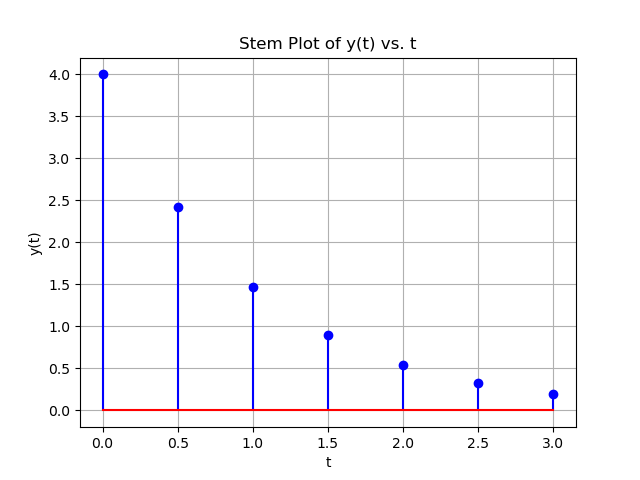
\includegraphics[width=1\linewidth]{\root\assign3\figs\plot.png}
     \caption{ plot of $\abs{V_{R}}$ vs  $t$}
 \end{figure}
 \begin{align}
2I\brak{s}-Li\brak{{0^{-}}}+LsI\brak{s}&=0\\
\implies I\brak{s}&=\frac{i\brak{{0^{-}}}}{s+2}\\
I\brak{s}&=\frac{2}{s+2}
 \end{align}
 applying inverse laplace transform
 \begin{align}
  i\brak{t}&=2e^{-2t} u\brak{t}\\
  V_R\brak{t}&=-2i\brak{t}u\brak{t}\\
  \implies V_R\brak{t}&=-4 e^{-2t} u\brak{t}
 \end{align}  
  As,
 \begin{align}
    t & \xrightarrow{} 0\\
     \implies e^{-2t}&\xrightarrow{} 1\\
     \abs{V_R\brak{max}}&=4
 \end{align}
\end{document}
